\documentclass[25pt, a0paper, portrait, margin=0mm, innermargin=15mm,blockverticalspace=2mm, colspace=5mm, subcolspace=4mm]{tikzposter}

\usepackage[utf8]{inputenc}

\usepackage{csquotes}
\usepackage[english]{babel}
\usepackage{lipsum}
\usepackage{fancyhdr}
\usepackage{amsmath,bm}
\usepackage{helvet}
\renewcommand\familydefault{\sfdefault}
\usepackage[T1]{fontenc}
\usepackage{transparent} % transparence des images
\usepackage{anyfontsize}
%\sethlcolor{} % couleur du surlignage

\usepackage[backend=biber,
    style=numeric-comp,
    maxcitenames=1,
    maxbibnames=1,
    %backref=true
    ]{biblatex}

\usepackage{colortbl} % colorer ligne d'un tableau
\usepackage{xspace}

\usepackage{tikz}
\usetikzlibrary{arrows,shapes}
\usepackage{pgfplots}

\usepackage{enumitem} % changer les points de itemize
\usepackage{environ}
\usepackage{adjustbox}

\tikzposterlatexaffectionproofoff %enlever phrase en bas à droite
\usetheme{Simple} %différents thèmes tikzposter

% ---- Couleurs
\definecolor{mypink1}{rgb}{0.858, 0.188, 0.478}
\definecolor{titlecolor}{RGB}{74, 114, 159}
\definecolor{titledarkcolor}{RGB}{51,102,153}
\definecolor{LightGrey}{RGB}{232, 232, 232}
\definecolor{Grey}{RGB}{222, 223, 225}
\definecolor{DarkerGrey}{RGB}{215,217,219}
\definecolor{FontColor}{RGB}{20,20,20}
\definecolor{Red}{RGB}{35, 135, 93}
\definecolor{L-lig}{RGB}{25,124,192}
\definecolor{point-lig}{named}{Red}
\definecolor{G-lig}{RGB}{62,66,68}


\definecolor{Orange}{RGB}{240,163,10}
\definecolor{Gray}{RGB}{186,200,211}
\definecolor{LightRed}{RGB}{214,98,93}
\definecolor{LightBlue}{RGB}{160,200,217}
\definecolor{LightGreen}{RGB}{130,161,119}
\definecolor{Violet}{RGB}{190,144,252}
% ----

\colorlet{blocktitlefgcolor}{Red} %titre des blocks
\colorlet{blocktitlebgcolor}{Grey} %couleur des lignes blocks
%\colorlet{blockbodybgcolor}{mypink1}%????
\colorlet{blockbodyfgcolor}{FontColor} %couleur du texte dans blocks
\colorlet{innerblocktitlebgcolor}{Red}
\colorlet{innerblocktitlebgcolor}{Red}
\colorlet{innerblocktitlefgcolor}{white}
\colorlet{notefrcolor}{Red!60} % ligne autour cadre notes
\colorlet{notefgcolor}{white} % couleur police notes
\colorlet{notebgcolor}{Red!60} % BG couleur des notes


% ---- Titre
\settitle{
\begin{minipage}[b]{0.7\linewidth}
\vspace{2cm}
\hspace{15mm}\color{white}{\Huge\textsc{\textbf{\@title}} \par }\vspace*{1cm} \hspace{15mm}\color{white}{\LARGE\@author \par}\vspace*{1cm}
\hspace{15mm}{\Large\@institute}\vspace{0.5cm}
\end{minipage}%
\hfill%
\begin{minipage}[b]{0.3\linewidth}
\hfill
\includegraphics[scale=1.1]{images/Logos/uhh-color.eps}\hspace{15mm}\vspace{0.5cm}
\end{minipage}
}



\definetitlestyle{sampletitle}{
width=840mm, roundedcorners=0, linewidth=2pt, innersep=15pt,
titletotopverticalspace=0mm, titletoblockverticalspace=-10mm
}{\begin{scope}[line width=\titlelinewidth, rounded corners=\titleroundedcorners]\draw[fill=point-lig, color=point-lig]
(\titleposleft,\titleposbottom) rectangle (\titleposright,\titlepostop);
\end{scope}}

\NewEnviron{posterbox}[1]
{\block[titleleft,roundedcorners=16]{#1}{\raggedright\BODY}}

\makeatletter
\newcounter{tablecounter}
\newenvironment{tikztable}[1][]{
  \def \rememberparameter{#1}
  \vspace{10pt}
  \refstepcounter{tablecounter}
  \begin{center}
  }{
    \ifx\rememberparameter\@empty
    \else
    \\[10pt]
    {\small Table~\thetablecounter: \rememberparameter}
    \fi
  \end{center}
}
\makeatother

\renewcommand{\arraystretch}{1.5}


\usepackage[font=small,skip=0.5ex]{caption}

\title{\parbox{1800pt}{A collaborative Web-Editor for Editing and Simulating Renew Reference Nets (Master's Thesis)}}

\author{{\underline{Laszlo Korte}\textsuperscript{1}}, Reviewer: {Dr. Daniel Moldt\textsuperscript{1}}, {Marcel Hansson\textsuperscript{1}}}
\institute{\textsuperscript{1}University of Hamburg, MIN-Fakultät, Fachbereich Informatik}

\usetitlestyle[]{sampletitle}
\setlength{\columnseprule}{0.3pt}

\addbibresource{masterarbeit.bib}
\addbibresource{tgi-temp.bib}

%%%%%%%%%%%%%%%%%%%%%%%%%%%%%%%%%%%%%%%%%%%%%%%%%%%%%%%%%%%
\begin{document}
\maketitle

% --- Lignes entre les colonnes

%------------------------------------------------------------------------------
% --------------------- CORPS DU POSTER ---------------------
%
\block{}{
}
\begin{columns}

\vspace{-1cm} % Adjust to your required vertical spacing
\column{0.5}

\begin{posterbox}{Introduction and Motivation}

 \LARGE
 \begin{itemize}

 \item Petri nets are a family of graphical modeling languages used for the specification and verification of concurrent processes and dynamic systems \cite{Petri77}.

 \item {\sc Renew} is a tool for the design and simulation of Petri nets and has been under continuous development at the University of Hamburg since 1999 \cite{Kummer+99}.

 \item However, {\sc Renew} cannot be used on mobile devices and does not support real-time collaborative editing by multiple users.

 \item \textbf{In this work} we present a web-based Petri net editor that enables collaborative editing and simulation on desktop and mobile devices, backed by the {\sc Renew} simulator.
 \end{itemize}


\end{posterbox}



\begin{posterbox}{Basics: Petri nets}

 \LARGE

 \begin{itemize}

 \item A net structure consists of passive elements (\textbf{places}; circular) and active elements (\textbf{transitions}; rectangular), which are connected by arrows (\textbf{arcs}).

 \item Places represent system states and containers for resources (\textbf{tokens}).

 \item Arcs and transitions represent actions and define the rules by which tokens may move from one place to another.

 \end{itemize}


\begin{tikzfigure}
    \centering
    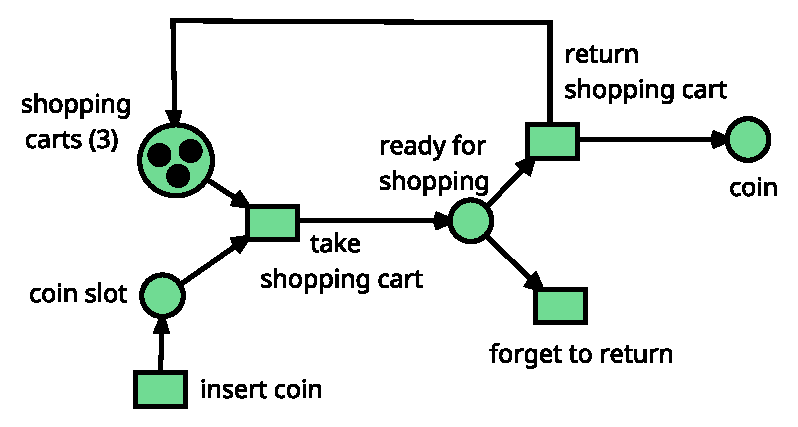
\includegraphics[scale=2.6]{images/ptnet-3.pdf}
    \captionof{figure}{%
        \small        % smaller font
        \linespread{1.5}\selectfont  % reduce line spacing
        Example of a Petri net consisting of 4 places, 4 transitions, and 3 tokens in one place, modeling a shopping cart rental system
    }
\end{tikzfigure}

\end{posterbox}

\begin{posterbox}{Requirements}

 \LARGE
 \begin{itemize}

     \item Existing {\sc Renew} files can be imported and exported.
     \item Documents support realtime collaborative editing.
     \item The editor runs in a web browser on various devices (desktops, smartphones, tablets).
     \item Complex Petri nets can be simulated using the powerful {\sc Renew} simulation engine.
     \item Interactive collaborative simulations are supported.

 \end{itemize}
\end{posterbox}


\column{0.5}

\begin{posterbox}{Implementation (System Architecture)}

 \LARGE
\begin{itemize}

    \item Client/Server architecture, communication via HTTP and WebSocket
  %  \item Documents are stored in a relational database (SQLite) on the server.
    \item Headless instances of {\sc Renew} are hosted on the central server for running the simulation.

\end{itemize}

\begin{tikzfigure}
    \centering
    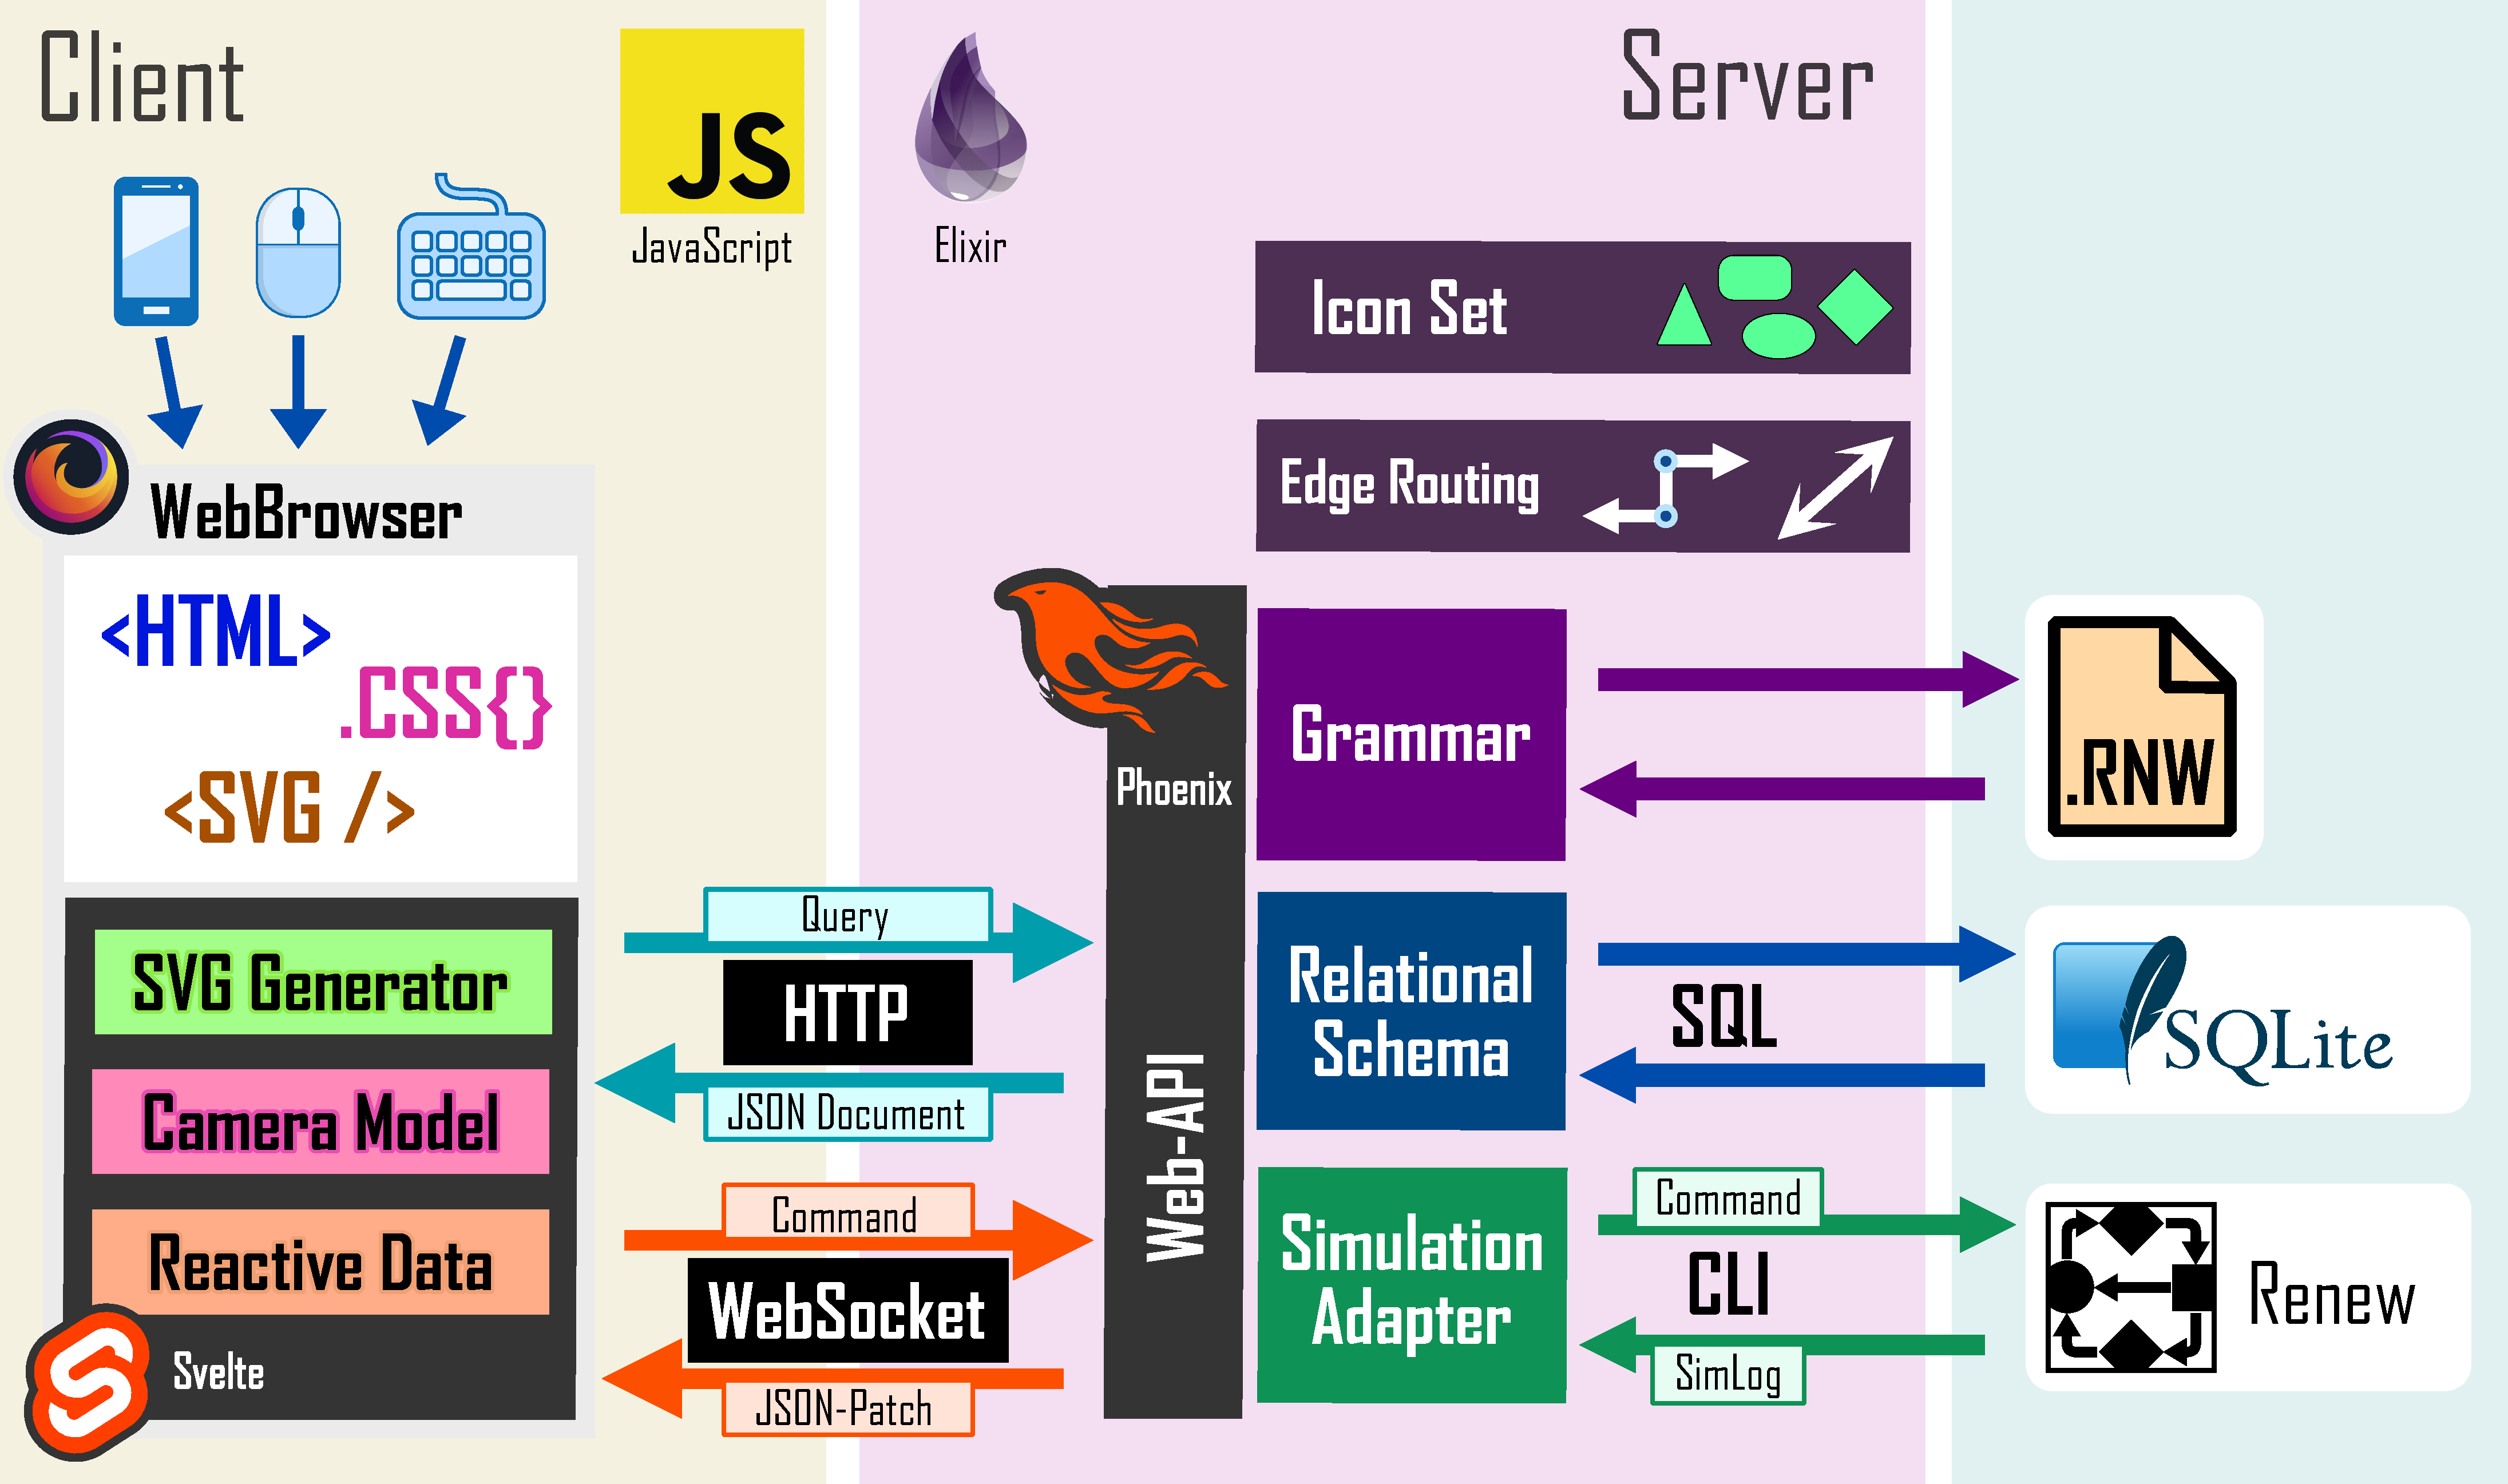
\includegraphics[trim={0 0cm 0 0cm},clip,scale=0.51]{images/petristation-architecture.pdf}
    \captionof{figure}{%
        \small        % smaller font
        \linespread{1.5}\selectfont  % reduce line spacing
        System architecture of the editor consisting of client and server components, with integration of {\sc Renew} and a relational database
    }
\end{tikzfigure}


\end{posterbox}

\begin{posterbox}{Result (User Interface)}

 \LARGE
\begin{itemize}
    \item The interactive canvas provides various tools for manipulating and navigating Petri nets.
\end{itemize}

\begin{tikzfigure}
    \centering
      %  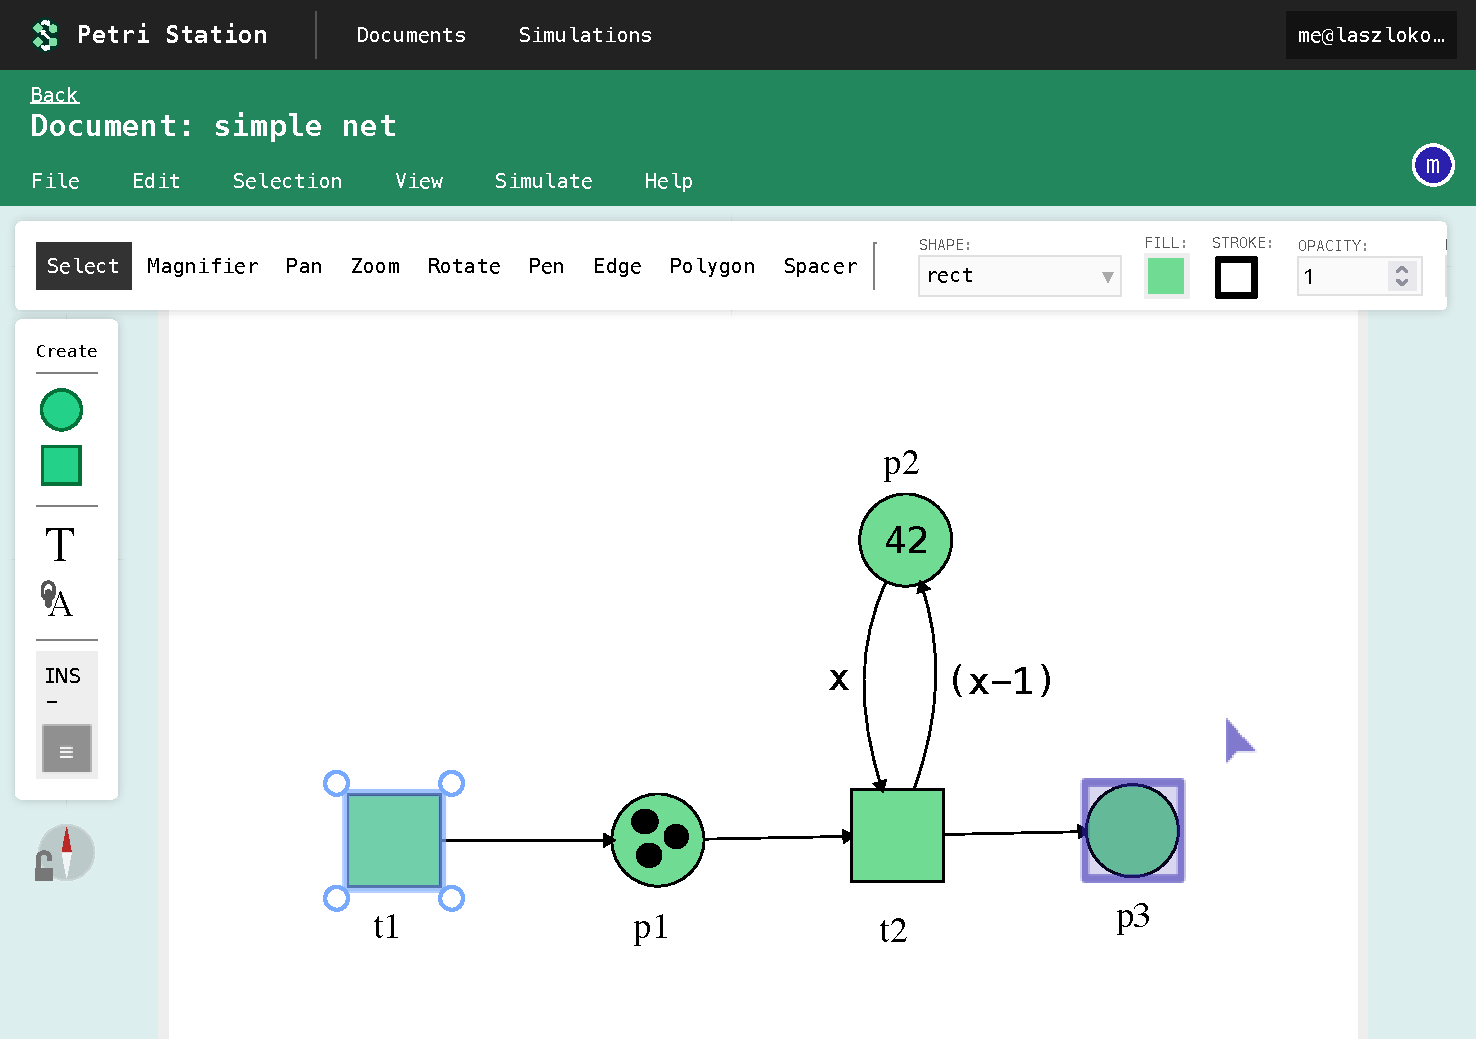
\includegraphics[trim={0 1cm 0 1cm},clip,scale=1.5]{images/remote.pdf}

    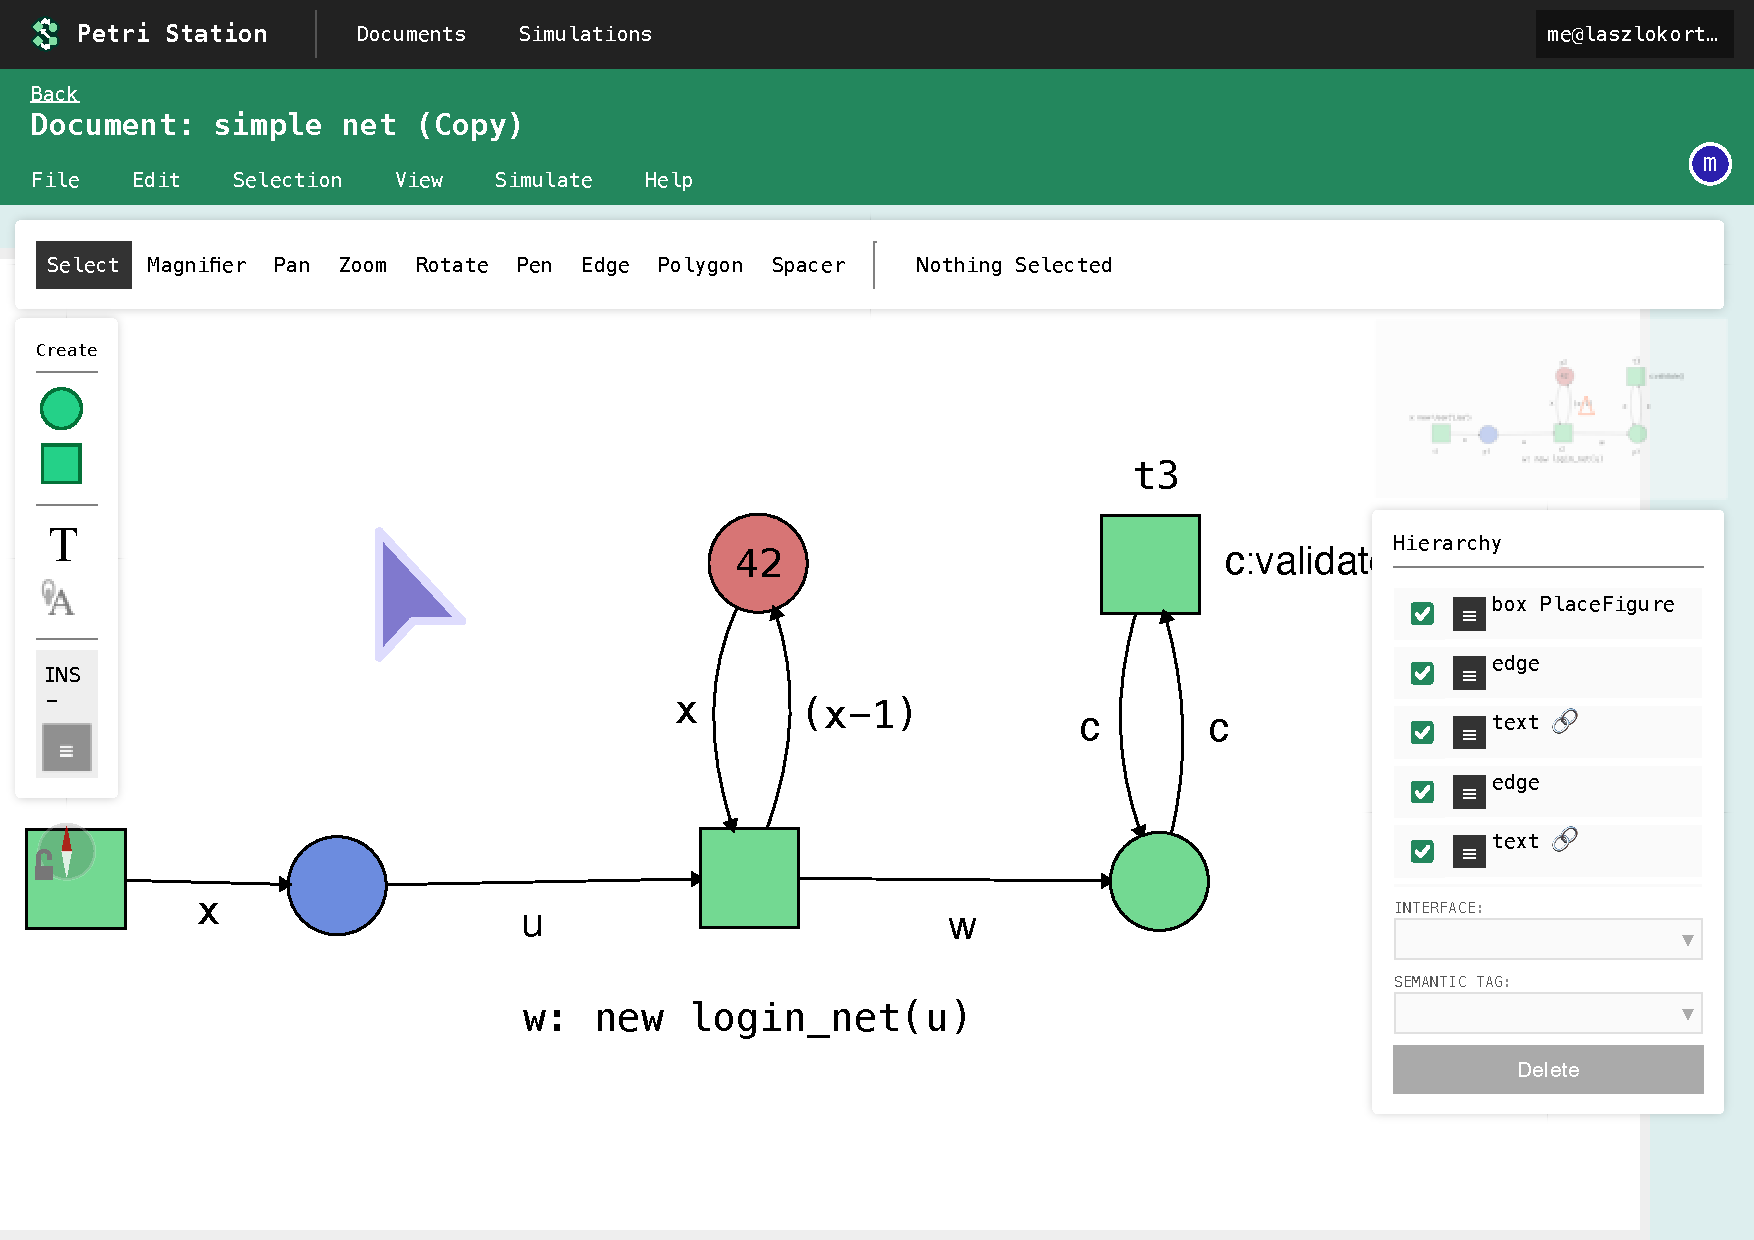
\includegraphics[trim={0 4.8cm 0 0},clip,scale=1.27]{images/PetriStation-document-3.pdf}

    \captionof{figure}{%
        \small        % smaller font
        \linespread{1.5}\selectfont  % reduce line spacing
        Screenshot of the editor user interface showing the toolbar (top), tool palette (left), mini-map(top right), element hierarchy (bottom right), and another user's collaborative cursor (center-left).
    }
\end{tikzfigure}

\end{posterbox}



\begin{posterbox}{Try it yourself!}
 \LARGE
\noindent
\begin{minipage}{0.24\linewidth}
  
\includegraphics[width=1\linewidth]{images/petri-qr.pdf}
\end{minipage}%
\hfill%
\begin{minipage}{0.72\linewidth}
  \Large
        Scan the QR code to access the web editor.
    \vspace{8mm}

  \noindent

  {\renewcommand{\arraystretch}{1.2}% for the vertical padding
  \begin{tabular}{ll}
   \multicolumn{2}{l}{ \url{https://editor.petristation.net}} \\
  \texttt{Login:    } & \texttt{   demo@tgi}\\
  \texttt{Password: } & \texttt{ petri2025}
  \end{tabular}}
\end{minipage}

\end{posterbox}
\begin{posterbox}{Outlook}
A follow-up Bachelor's thesis with significant improvements is currently in progress.
\end{posterbox}
       \end{columns}
\raisebox{2.9cm}[0pt][0pt]{%
       \begin{posterbox}{References}

   \printbibliography[heading=none]
   \end{posterbox}
   }


% ----------------- Ligne colorée à la fin du document -------------
\node [above right, text=white,inner sep=15pt,outer sep=45pt,minimum width=\paperwidth, align=center, draw, fill=titledarkcolor, color=point-lig] at (-43.6,-61) { \textcolor{white}{\normalsize Laszlo Korte --- University of Hamburg, 2025}};

%\node [text=white,outer sep=45pt, align=center, draw,fill=FontColor,circle, above left] at (41,-57) {\Large \#54};

\node [text=white,outer sep=45pt, align=center, below left] at (42,60) {
\includegraphics[scale=0.55]{images/Logos/petristation-logo.pdf}};


\end{document}
